\documentclass[standalone]{beamer}

\begin{document}
\section{數論}

\begin{frame}{\btitle{目標}}
  \begin{problem}[An Easy Problem, NTUJ 1423]
    給你等式 $a^b \equiv c \pmod{d}$ 中的其中 $3$ 個,請計算出剩下的一個。\\
    (不同的子題有不同的範圍)
  \end{problem}
\end{frame}

\begin{frame}{\btitle{基礎}}
  %\bigskip
  %\begin{enumerate}
    %\item $a^b \equiv \raisebox{-.2mm}{\text{?}} \pmod{d}$: 快速冪,$\ord(\log b)$。
  %\end{enumerate} \vspace{-1em} \pause
  %\begin{minted}{cpp}
%int fastpow(int a, int b, int m) {
    %if (!b) return 1%m;
    %int ret = fastpow(a*a%m, b/2, m);
    %if (b&1) (ret *= a) %= m;
    %return ret;
%}
  %\end{minted}
  \begin{problem}[An Easy Problem -- Subtask \#1, NTUJ 1423]
    給你 $a$, $b$,求最大的 $m$ 使得 $a \equiv b \pmod{m}$。 ($a, b \leq 10^{12}$)
  \end{problem} \pause

  \begin{definition} \vspace{-0.5\baselineskip}
    \[ a \equiv b \pmod{m} \iff a - b \mid m \]
  \end{definition}
\end{frame}

\begin{frame}[fragile]{\btitle{基礎}}
  \begin{problem}[An Easy Problem -- Subtask \#2, NTUJ 1423]
    給你 $a$, $b$, $m$,求 $c \equiv a^b \pmod{m}$。 ($0 \leq a < m \leq 10^{9}$, $b \leq 10^{12}$)
  \end{problem} \pause \disskip
  快速冪 ($\ord(\log n)$): \disskip
  \begin{itemize}[<+->]
    \item 如果 $b = 2b'$,則 $a^b \equiv \big( a^{b'} \big)^2 \pmod{m}$。
    \item 如果 $b = 2b' + 1$,則 $a^b \equiv a \cdot \big( a^{b'} \big)^2 \pmod{m}$。
  \end{itemize} \disskip
  \definecolor{haohao}{rgb}{0.69,0.00,0.25}
  \onslide<+->
  \begin{minted}[escapeinside=αα]{cpp}
long long fpow(long long a, long long b, α\textcolor{haohao}{\textbf{long 1ong}}α m) [
    if (!a) return 1;
    int ret = fastpow(a*a, b/2, m);
    if (b&1) (ret *= b) %= m;
   return ret; α\textcolor{gray}{\textbackslash\textbackslash return a**b % m}α
}
  \end{minted}
\end{frame}

\begin{frame}{\btitle{基礎}}
  \begin{problem}[An Easy Problem -- Subtask \#3, NTUJ 1423]
    給你 $a$, $c$, $m$,求 $b$ 使得 $a^b \equiv c \pmod{m}$。\\
    ($a, b, m \leq 10^{9}$, $m$ 是質數)
  \end{problem} \pause \disskip
  \[ a^{xk + y} \equiv c \pmod{m} \iff a^{xk} \equiv c a^{-y} \pmod{m} \]
  \pause \disskip
  \begin{enumerate}
    \item 取 $k \defeq \lfloor \sqrt{m} \rfloor$。
    \item 找 $\{a^{xk}\}$, $\{c a^{-y}\}$ 有沒有一樣的元素。
  \end{enumerate}
  \pause
  \begin{missue}
    \centering
    怎麼求出 $a^{-1} \bmod m$?
  \end{missue}
\end{frame}

\begin{frame}{\btitle{模逆元}}
  也就是要找 $b$ 使得
  \[ a b \equiv 1 \pmod{m} \onslide<+(1)->{\implies \exists k',\, ab = k'm + 1 \implies \exists k,\, ba + km = 1}\]
  \pause \disskip
  \begin{theorem}[$ax + by = 1$ 有解的條件] \vspace*{-0.5\baselineskip}
    \[ ax + by = 1 \ \text{有解} \iff \gcd(a, b) = 1 \]
  \end{theorem}
  \pause \disskip
  \begin{enumerate}[<+->]
    \item 假設 $a = kb + r, \ 0 \leq r < b$,並且我們已經知道 
      \begin{equation}
        bx' + ry' = 1 \label{eq:gcd}
      \end{equation}
    \item 把 $r = a - kb$ 代入 \eqref{eq:gcd} 我們得到 $y'a + (x' - ky')b = 1$。
  \end{enumerate}
\end{frame}

\begin{frame}{\btitle{模逆元}}
  \begin{theorem}[模逆元存在的條件]
   模 $m$ 下 $a^{-1}$ 存在 $\iff \gcd(a, m) = 1$。
  \end{theorem}
  \pause

  我們把在模 $m$ 下與 $m$ 互質的所有數的集合稱作模 $m$ 的\emph{乘法群},寫作
  \[ (\bZ / m\bZ)^\times \defeq \{ a \mid 0 \leq a < m,\, \gcd(a, m) = 1 \} \]
  \pause
  \begin{missue}
    \centering
    $(\bZ / m\bZ)^\times$ 長什麼樣子?
  \end{missue}
\end{frame}

\begin{frame}{\btitle{乘法群}}
  \begin{missue}
    \centering
    $(\bZ / m\bZ)^\times$ 有多少個元素?
  \end{missue}
  \pause \disskip

  也就是有多少個 $0 \leq a < m$ 使得 $\gcd(a, m) = 1$? \\[\parskip]
  \pause

  \begin{definition} \vspace*{-1em}
    \[ \varphi(m) = \sharp \{ a \mid 0 \leq a < m, \, \gcd(a, m) = 1\} \]
  \end{definition}
  \pause \disskip
  顯然對於質數,$\varphi(p) = p-1$。 \\ \pause
  那對於 $\gcd(p, q) = 1$,$\varphi(p q)$ 呢?
\end{frame}

\begin{frame}{\btitle{韓信點兵}}
  「相傳漢高祖劉邦有天趁喝酒的時候問大將軍韓信統御兵士多少,
韓信答說,每 $3$ 人一列餘 $1$ 人、 $4$ 人一列餘 $2$ 人、$5$ 人一列餘 $4$ 人。
劉邦與張良都算不出來,以為韓信兵很多,嚇到吃手手。」
\pause

其實就是要解
\[
  \begin{cases}
    x \equiv 1 \pmod{3} \\
    x \equiv 2 \pmod{4} \\
    x \equiv 4 \pmod{5} \\
  \end{cases}
\]
\end{frame}

\begin{frame}{\btitle{中國剩餘定理}}
  \begin{theorem}[中國剩餘定理]
    如果 $m_1, m_2, \dots, m_n$ \alert<1>{互質},則
    \[
      \begin{cases}
        x \equiv a_1 \pmod{m_1} \\
        x \equiv a_2 \pmod{m_2} \\
        \quad \quad \vdots \\
        x \equiv a_n \pmod{m_n} \\
      \end{cases}
    \]
    有解,\onslide<2->{且解為
      \[ x \equiv a_1 t_1 M_1 + a_2 t_2 M_2 + \dots + a_n t_n M_n \pmod{m_1 m_2 \dotsm m_n} \]
      其中 $M_i \defeq \prod_j m_j / m_i = \prod_{j \neq i} m_j$, $t_i \defeq M_i^{-1} \bmod m_i$。
    }
  \end{theorem}
\end{frame}

\begin{frame}{\btitle{中國剩餘定理}}
  \begin{theorem}[中國剩餘定理]
    如果 $m_1, m_2, \dots, m_n$ 互質,則
    \[ \psi(x) = (x \bmod m_1, x \bmod m_2, \dots, x \bmod m_k) \]
    是一個一對一且滿射的函數,且
    \[
      \bZ / m\bZ \,\cong\, \bZ / m_1 \bZ \tikzoverlay{ch_m1}{$\:\times\:$} \bZ / m_2 \bZ \tikzoverlay{ch_m2}{$\:\times\:$} \dots \times \bZ / m_k \bZ
    \]
  \end{theorem}
  \pause

  \visible<+->{
    \begin{tikzpicture}[overlay, remember picture]
      \node[inner sep=0.2ex] (txt) at ($(ch_m1) + (-1, -1.5)$) {\cppinline[fontsize=\ofootnotesize]{std::tuple<T, U, ...>}};
      \path[->] (txt.north) edge[out=70, in=260] (ch_m1.south);
      \path[->] (txt.north) edge[out=60, in=230] (ch_m2.south);
    \end{tikzpicture}
  }
\end{frame}

\begin{frame}{\btitle{Euler $\varphi$}}
  \begin{theorem}
    假設 $n, m$ 互質,則 $\varphi(nm) = \varphi(n) \varphi(m)$。
  \end{theorem}
  \pause

  \begin{proof}
    \begin{enumerate}[<+->]
      \item 因為 $\gcd(a, nm) = 1$ $\iff \gcd(a, n) = 1 \ \text{且} \gcd(a, m) = 1$。
      \item 每個滿足 $\gcd(x, n) = 1$ 且 $\gcd(y, m) = 1$ 的數對 $(x, y)$ 由中國剩餘定理
        又可以對回模 $nm$ 下的一個數。
      \item 這樣的數對有 $\varphi(n) \varphi(m)$ 個。
    \end{enumerate}
  \end{proof}
\end{frame}

\begin{frame}{\btitle{Euler $\varphi$}}
  \begin{itemize}[<+->]
    \item $\varphi(p) = p-1$。
    \item $\varphi(p^k) = p^{k-1}(p-1)$。
  \end{itemize}

  \onslide<+->
  \begin{theorem}
    如果 $n = p_1^{\alpha_1} p_2^{\alpha_2} \dotsm p_k^{\alpha_k}$,則
    \[
      \begin{aligned}
        \varphi(n) &= p_1^{\alpha_1-1} (p_1 - 1) p_2^{\alpha_2-1}(p_2 - 1) \dotsm p_k^{\alpha_k-1}(p_k - 1) \\
        &= n \prod_{p \mid n} \left( 1 - \frac{1}{p} \right)
      \end{aligned}
    \]
  \end{theorem}
\end{frame}

\begin{frame}{\btitle{題目}}
  \begin{problem}[Cool lucky function, {\small NTU final 2014}]
    給你 $n$ 個正整數 $a_1, a_2, \dots, a_n$,問你這些數字之中是否存在兩個互質的數對。
    ($2 \leq n \leq 10^5, \, a_i \leq 10^6$)
  \end{problem}
\end{frame}

\begin{frame}{\btitle{趣事}}
  \begin{problem}[數學歸納法考題]
    令 $x_1 = 1$, $x_{n+1} = 2x_n + 1$,請證明 $x_{n} \leq 2^n - 1$。
  \end{problem} \pause
  \begin{proof}
    \begin{itemize}[<+->]
      \item $n = 1$ 時顯然成立。
      \item 假設 $n = k$ 時成立,$x_{k+1} = 2x_k + 1 \leq 2\cdot(2^k - 1) + 1 = 2^{k+1} - 1$。
      \item 由數學歸納法證畢。
    \end{itemize}
  \end{proof}
\end{frame}

\begin{frame}{\btitle{趣事}}
  結果老師打錯一個字:
  \begin{problem}[數學歸納法考題 -- 錯誤版]
    令 $x_1 = 1$, $x_{n+1} = 2x_n + 1$,請證明 $x_{n} \leq 2^n \alert<1>{+} 1$。
  \end{problem} \pause
  \begin{proof}
    \begin{itemize}[<+->]
      \item $n = 1$ 時顯然成立。
      \item 假設 $n = k$ 時成立,$x_{k+1} = 2x_k + 1 \leq 2\cdot(2^k + 1) + 1 = 2^{k+1} + 3 \nleq 2^{k+1} + 1$。
      \item ?????
    \end{itemize}
  \end{proof}
\end{frame}

\begin{frame}{\btitle{題目}}
  有時候題目變難,反而好做! \pause

  \begin{problem}[Cool lucky function -- Hard]
    給你 $n$ 個正整數 $a_1, a_2, \dots, a_n$,問你這些數字之中\alert<2>{有多少對互質的數對}。
    ($2 \leq n \leq 10^5, \, a_i \leq 10^6$)
  \end{problem} \pause
  排容:令 $c_k \defeq \sharp\{ (a, b) : k \mid \gcd(a, b) \}$。\pause

  要算的是
  \[ 
    \frac{n(n-1)}{2} - \sum_{p \text{ prime}} c_p + \sum_{p,q \text{ prime}} c_{pq} - \dotsm
  \]
\end{frame}

\begin{frame}{\btitle{乘法群}}
  \begin{missue}
    \centering
    $(\bZ / m\bZ)^\times$ 長什麼樣子?
  \end{missue}
  \pause

  我們只要會 $(\bZ / p^k \bZ)^\times$ 就可以了,其中 $p$ 是質數。
  \pause

  先看 $(\bZ / p \bZ)^\times$。
\end{frame}

\begin{frame}{\btitle{乘法群}}
  \begin{figure}
    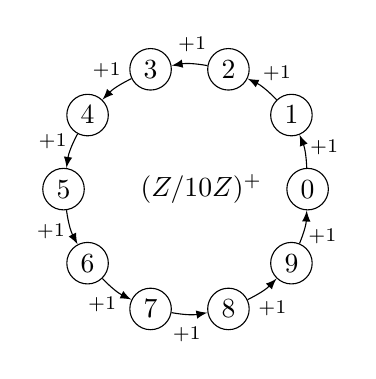
\begin{tikzpicture}[
        nd/.style={draw, circle, inner sep=0.2ex, minimum size=1.5em},
      ]
      \foreach \x [count=\i] in {36,72,...,324} {
        \node (v\i) at (\x:1.6) [nd] {$\i$};
      }
      \node (v0) at (0:1.5) [nd] {$0$};
      \foreach \x [count=\i from 2] in {3,4,...,9} {
        \pgfmathsetmacro\shang{10+36*\i}
        \path[-latex, draw] (v\i) edge[bend right=10] node[shift=(\shang:0.25)]{\scriptsize $+1$} (v\x);
      }
      \foreach \x/\i in {9/0,0/1,1/2} {
        \pgfmathsetmacro\shang{10+36*\x}
        \path[-latex, draw] (v\x) edge[bend right=10] node[shift=(\shang:0.25)]{\scriptsize $+1$} (v\i);
      }
      \node at (0.15, 0) {$(\mathbb{Z} / 10 \mathbb{Z})^+$};
    \end{tikzpicture}
    \quad
    \onslide<2->{
    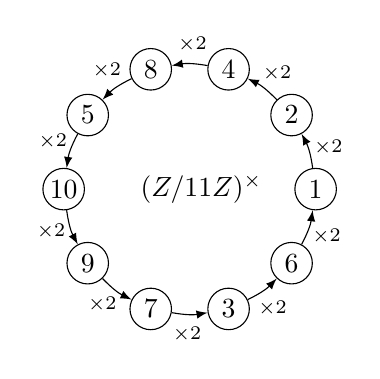
\begin{tikzpicture}[
        nd/.style={draw, circle, inner sep=0.2ex, minimum size=1.5em},
      ]
      \foreach \c/\x [count=\i from 0] in {
        1/0,
        2/36,
        4/72,
        8/108,
        5/144,
        10/180,
        9/216,
        7/252,
        3/288,
        6/324
      } {
        \node (v\i) at (\x:1.6) [nd] {$\c$};
      }
      \foreach \x [count=\i from 2] in {3,4,...,9} {
        \pgfmathsetmacro\shang{10+36*\i}
        \path[-latex, draw] (v\i) edge[bend right=10] node[shift=(\shang:0.25)]{\scriptsize $\times 2$} (v\x);
      }
      \foreach \x/\i in {9/0,0/1,1/2} {
        \pgfmathsetmacro\shang{10+36*\x}
        \path[-latex, draw] (v\x) edge[bend right=10] node[shift=(\shang:0.25)]{\scriptsize $\times 2$} (v\i);
      }
      \node at (0.15, 0) {$(\mathbb{Z} / 11 \mathbb{Z})^\times$};
    \end{tikzpicture}
    }
  \end{figure}
  \onslide<3-> {
    $\implies$ 模 $11$ 下的乘法等同於模 $10$ 下的加法。
  }
\end{frame}

\begin{frame}{\btitle{原根}}
  %\begin{definition}[階]
    %定義 $n \defeq \operatorname{ord}_m(a)$ 為最小的正整數 $n$ 使得 $a^n \equiv 1 \pmod{m}$。
  %\end{definition}
  %\pause

  \begin{definition}[原根]
    如果 $a^k$ 遍歴所有 $(\bZ / m \bZ)^\times$ 下的元素,我們就說 $a$ 是一個\emph{原根}。
  \end{definition}
  \pause

  \begin{theorem}[原根存在的條件]
    原根存在若且唯若 $m = 1, 2, 4, p^k, 2p^k$。
  \end{theorem}
\end{frame}

\begin{frame}{\btitle{Euler 定理}}
  \begin{theorem}[Euler 定理]
    \begin{itemize}
      \item 對於質數 $p$,$a^{p-1} \equiv 1 \pmod{p}$。
      \item 對於任何數 $m$,$a^{\varphi(m)} \equiv 1 \pmod{m}$。
    \end{itemize}
  \end{theorem}
  \pause \disskip

  \[ a \cdot a^{\varphi(m) - 1} \equiv 1 \pmod{m} \implies a^{-1} \equiv a^{\varphi(m) - 1} \pmod{m} \]
\end{frame}

\begin{frame}{\btitle{RSA}}
  \begin{enumerate}[<+->]
    \item \alert<7>{選兩個大質數 $p, q$}。
    \item \alert<6>{令 $r = \varphi(pq) = (p-1)(q-1)$}。
    \item 選 $e$ 使得 $\gcd(e, r) = 1$,此時 $e$ 在模 $r$ 下有反元素 $d$。
    \item 加密 $x \to x^e$。
    \item 解密 $(x^e)^d \to x^{ed} \equiv x \pmod{pq}$。
  \end{enumerate}

  \begin{itemize}[<+->]
    \item 我們無法快速分解因數。
    \item 但可以快速判斷質數!
  \end{itemize}
\end{frame}

\begin{frame}{{\secname}}
  競賽常用的演算法:\pause
  \begin{itemize}
    \item 判斷 $n$ 是不是質數:Miller Rabin $ \implies \ord\big(\log^{\ord(1)}(n)\big)$
    \item 因數分解 $n$ :Pollard's rho $ \implies \ord(n^{1/4})$
  \end{itemize}
\end{frame}

\begin{frame}{\btitle{找循環節}}
  \begin{problem}[找循環節]
    給你一個函數 $f$ 和 $x_0$,對於所有 $i \geq 1$ 令 $x_i \defeq f(x_{i-1})$,
    找出 $i \neq j$ 使得 $x_i = x_j$。
  \end{problem}
  \pause

  \begin{enumerate}[<+->]
    \item 令 $x = y = x_0$。
    \item 每次 $x \gets f(x)$, $y \gets f(f(y))$。
    \item 有循環節的話總是會找到。
  \end{enumerate}
\end{frame}

\begin{frame}{\btitle{生日悖論}}
  現在有 $70$ 個人,生日都在 $3 \cdot 365$ 天的範圍內。假設每個人的生日是獨立的,
  有 $99\%$ 的機率兩個人同年同月同日生! \pause

  假設有 $n$ 個人,隨機選 $m$ 個位置。\\ \pause
  任兩個人同個位置的機率是 $1 / m$。 \\ \pause
  令 $X$ 表示有多少對人是同一個位置
  \[ \implies \Expect[X] = \frac{n(n-1)}{2} \frac{1}{m} \]
  \pause
  $n^2 \approx m \implies n = \ord(\sqrt{m})$ 時就有高機率相撞!
\end{frame}

\begin{frame}{\btitle{生日悖論應用}}
  用 Hash 解以下兩題:
  \begin{problem}
    給你 $n$ 個字串,問其中有沒有字串和 $A$ 相等。
  \end{problem}
  \pause
  \begin{problem}
    給你 $n$ 個字串,問其中有沒有兩個字串相等。
  \end{problem}
  \pause
  Hash 的值分別要超過 $\ord(n), \ord(n^2)$。
\end{frame}

\begin{frame}{\btitle{期望值}}
  期望值有一個好性質:
  \begin{theorem} 如果 $X, Y$ 是兩個隨機變數,\alert<1>{不論 $X, Y$ 是否獨立},都有
  \[
    \Expect[aX + Y] = a\Expect[X] + \Expect[Y] \label{eq:expect_linear}
  \]
  \pause
  \end{theorem}
  這常是解題的關鍵
\end{frame}

\begin{frame}{\btitle{期望值}}
  \begin{problem}[Graph Game, Codeforces 235D]
    現在有一個遊戲: \pause
    \begin{enumerate}[<+->]
      \item 一開始的分數是 $0$,並且有一個 $n$ 個點的樹。
      \item 每次從剩下的點中隨機且等機率的選出一個點 $v$,並把分數加上 $v$ 所在的
        連通塊的大小,且把 $v$ 和與 $v$ 相鄰的邊全部刪掉。
      \item 一直進行到圖上沒有點為止。
    \end{enumerate}

    \onslide<+->
    問你得到的分數的期望值。
  \end{problem}
\end{frame}

\begin{frame}{\btitle{期望值}}
  改求 $u$ 被拔掉時 $u, v$ 還連通的機率。 \pause
  \begin{figure}
    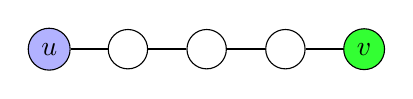
\begin{tikzpicture}[every node/.style={circle, draw, minimum size=5mm, inner sep=1mm}]
      \node(1) at (0, 0) {};
      \node(2) at (1, 0) {};
      \node[fill=green!80] (3) at (2, 0) {$v$};
      \node(4) at (-1, 0) {};
      \node[fill=blue!30] (5) at (-2, 0) {$u$};
      \draw (1) edge[thick] (2);
      \draw (3) edge[thick] (2);
      \draw (1) edge[thick] (4);
      \draw (5) edge[thick] (4);
    \end{tikzpicture}
  \end{figure} \pause

  等價於 $u$ 是這些點中第一個被拔掉的點 \pause。 \\
  $\implies p = 1/n$,$n$ 是 $u, v$ 間(包含)有幾個點。
\end{frame}

\begin{frame}[fragile]{\btitle{Pollard's rho}}
  \begin{minted}{cpp}
    int f(int x, int n) { return (x*x + 2) % n }
    int pollard_rho(int n) {
        int xi, xj;
        int i = 1, j = 1;
        xi = xj = 2;
        while (true) {
            j++;
            xi = f(xi, n);
            xj = f(f(xj, n));
            int d = __gcd(abs(xi - xj), n);
            if (d != 1) return d;
        }
    }
  \end{minted}
\end{frame}

\begin{frame}{\btitle{Pollard's rho}}
  假設 $n = pq$ \pause
  \begin{enumerate}[<+->]
    \item 用偽隨機函數 $f$ 生成序列 $x_0, x_1, \dots $。
    \item 當產生的數 $n \equiv \sqrt{p}$ 時應該就會有 $x_i \equiv x_j \pmod{p}$,
      也就是 $x_i \pmod{p}$ 在循環了。
    \item 令 $g \defeq \gcd(x_i - x_j, n)$,因為 $p, q$ 互質不太可能也剛好 $x_i \equiv x_j \pmod{q}$,
      所以 $g$ 高機率會是一個真因數。
  \end{enumerate}
\end{frame}

\begin{frame}{\btitle{Final}}
  \begin{problem}[An Easy Problem -- Subtask \#4, NTUJ 1423]
    給你 $b$, $c$, $p$,請你求 $a$ 使得 $a^b \equiv c \pmod{p}$。\\
    ($b, c, p \leq 10^9$, $p$ 是數且 $\gcd(b, p-1) \leq 10^5$)
  \end{problem} \pause

  請看講義…
\end{frame}
\end{document}
